% !TEX root = handbook-physics.tex
% !TEX TS-program = pdflatex
% !TEX encoding = UTF-8 Unicode






\chapter{Fundamentals of Maxwell's Theory}
\label{ch-27}
\zhtitle{麦克斯韦理论基础}

\section{General Features of Maxwell's Theory}
\label{sec-27.1}
\zhtitle{麦克斯韦理论的一般特征}


\subsection{}\label{27.1.1} \redem{Maxwell's theory} is a systematic theory of a unified electromagnetic field \ssect{15.1.2} set up by an arbitrary system of charges and currents. Maxwell's theory enables the \redem{principal problem of electrodynamics} to be solved: determining the characteristics of electric and magnetic fields on the basis of a given distribution of charges and currents that set up these fields. Maxwell's theory is a generalization of fundamental laws that describe electrical and electromagnetic phenomena. These include the Ostrogradsky-Gauss theorem \ssect{18.3.3}, the total cur­ rent law \ssect{26.4.2}, and the law of electromagnetic induction \ssect{25.1.2}.
\zhpar{\redem{麦克斯韦理论}是描述由任意电荷和电流系统所激发的统一电磁场的系统理论。麦克斯韦理论使\redem{电动力学的基本问题}得以解决，即根据激发电场和磁场的已知电荷与电流分布，确定电场和磁场的特征。麦克斯韦理论是对描述电现象和电磁现象的基本定律的推广，其中包括奥斯特罗格拉茨基-高斯定理（见\ssect{18.3.3}）、全电流定律（见\ssect{26.4.2}）以及电磁感应定律（见\ssect{25.1.2}）。}

\subsection{}\label{27.1.2} Maxwell's theory is of a phenomenological nature. This is manifested in the fact that it does not deal with the internal mechanism of the phenomena that occur in a medium and lead to the production of electric and magnetic fields. The medium is described in this theory by three quantities that specify its electrical and magnetic properties. These are the relative permittivity (dielectric constant) $\varepsilon_{r}$ \ssect{18.3.4}, relative magnetic permeability $\mu_{r}$ \ssect{26.4.5} and the electrical conductivity $\varkappa$ \ssect{20.3.4}.
\zhpar{麦克斯韦理论具有唯象性质，这表现为它不研究介质中产生电场和磁场的现象的内部微观机制。在该理论中，介质由三个描述其电学和磁学性质的量来表征，即相对电容率（相对介电常量）$\varepsilon_{r}$（见\ssect{18.3.4}）、相对磁导率 $\mu_{r}$（见\ssect{26.4.5}）以及电导率 $\varkappa$（见\ssect{20.3.4}）。}

\subsection{}\label{27.1.3} Maxwell's theory deals with macroscopic fields set up by macroscopic charges and currents that are concentrated in volumes incommensurably greater than those of atoms (or molecules). It is assumed that the distances from the sources of the fields to the points in space being considered substantially exceed the linear dimensions of atoms (or molecules). Therefore, macroscopic fields change appreciably only at distances that are huge compared to the linear dimensions of atoms (or molecules). Moreover, the periods of time required for changes in variable electric and magnetic fields are considered to be considerably longer than those required for intra-molecular processes.
\zhpar{麦克斯韦理论讨论的是由宏观电荷和宏观电流激发的宏观场，这些宏观电荷和宏观电流集中在远大于原子（或分子）体积的区域内。假定场源到所考察空间点的距离远大于原子（或分子）的线度，因此宏观场只在远大于原子（或分子）线度的距离上才有明显变化。此外，认为变化的电场和磁场发生变化所需的时间远长于分子内部过程所需的时间。}

\subsection{}\label{27.1.4} The macroscopic charges and currents are the sets of microscopic charges and currents that set up their micro-fields (electric and magnetic), varying continuously with time at each point in space.
\zhpar{宏观电荷与宏观电流是由微观电荷与微观电流的集合构成的，这些微观电荷与微观电流在空间各点激发微观场（电场和磁场），且该微观场随时间连续变化。}

The macroscopic fields dealt with in Maxwell's theory are \redem{averaged micro-fields}. Averaging is carried out over time intervals considerably longer than those typical of inter-atomic processes, and over volumes of fields many times greater than the volumes of atoms and molecules \ssect{27.4.5}.
\zhpar{麦克斯韦理论中的宏观场是\redem{平均微观场}。取平均所用的时间间隔远长于原子间过程的典型时间，所取的体积比原子和分子的体积大许多倍（参见\ssect{27.4.5}）。}

\subsection{}\label{27.1.5} Maxwell's theory is one of \redem{short-range action}, according to which electrical and magnetic interactions take place in electric and magnetic fields and propagate at a finite velocity equal to that of light in the given medium. This important consequence is taken into account in the electromagnetic theory of light developed by Maxwell.
\zhpar{麦克斯韦理论属于\redem{近距作用}理论：电相互作用和磁相互作用通过电场和磁场进行，并以有限速度传播，其传播速度等于给定介质中的光速。麦克斯韦所建立的光的电磁理论考虑了这一重要结论。}



\section{Maxwell's First Equation}
\label{sec-27.2}
\zhtitle{麦克斯韦第一方程}


\subsection{}\label{27.2.1} Maxwell's first equation in integral form is a generalization of Faraday's law of electromagnetic induction in the form \ssect{25.1.2}:
\zhpar{麦克斯韦第一方程的积分形式是对法拉第电磁感应定律（其形式见\ssect{25.1.2}）的推广：}
\begin{align*}%
\oint_{L} \vb{E}\, \dd \vb{l} & = - \pdv{\Phi_{m}}{t} && \text{(in SI units),} \\
\oint_{L} \vb{E}\, \dd \vb{l} & = - \frac{1}{c} \pdv{\Phi_{m}}{t} && \text{(in Gaussian units)},
\end{align*}
According to Maxwell, this law is valid for any closed circuit, or loop, and hot only current-conducting ones, conceivably selected in a variable magnetic field. This means that a variable magnetic field sets up a rotational electric field at any point in space, regardless of whether or not there is a conductor at that point.
\zhpar{按照麦克斯韦的观点，该定律适用于任意闭合回路（即闭合环路），而不仅限于导电回路，这些回路可以设想为置于变化磁场中的任意回路。这意味着，变化的磁场会在空间任一点激发涡旋电场，而与该点是否存在导体无关。}

\subsection{}\label{27.2.2} Using the following expression for the magnetic flux \ssect{23.5.5}:
\zhpar{利用磁通量的如下表达式（见\ssect{23.5.5}）：}
\begin{equation*}%
\Phi_{m} = \oint_{S} \vb{B}\, \dd S = \oint_{S}{B}_{n}\, \dd S,
\end{equation*}
and the Stokes theorem from vector analysis:
\zhpar{并利用矢量分析中的斯托克斯定理：}
\begin{equation*}%
\oint_{S} \vb{E}\, \dd \vb{l} = \oint_{S} \curl \vb{E}\, \dd \vb{S},
\end{equation*}
where $\dd \vb{S} = \vu{n}\, \dd S$ ($\vu{n}$ being the unit vector of the normal to the element $\dd S$ of surface), we can convert Maxwell's first equation as given in \ssect{27.2.1} to \redem{Maxwell's first equation in differential form}:
\zhpar{式中 $\dd \vb{S} = \vu{n}\, \dd S$（$\vu{n}$ 为面元 $\dd S$ 的法线单位矢量），于是可将\ssect{27.2.1}中给出的麦克斯韦第一方程化为\redem{麦克斯韦第一方程的微分形式}：}
\begin{align*}%
\curl \vb{E} & = - \pdv{\vb{B}}{t} && \text{(in SI units),} \\
\curl \vb{E} & = - \frac{1}{c}\pdv{\vb{B}}{t}&& \text{(in Gaussian units)},
\end{align*}
Here $\curl \vb{E}$ is expressed in Cartesian coordinates by the determinant
\zhpar{这里 $\curl \vb{E}$ 在笛卡儿直角坐标系中由下列行列式表示：}
\begin{equation*}%
\curl \vb{E} = \mdet{\vu{i} & \vu{j} & \vu{k}\\ \pdv{x} & \pdv{y} & \pdv{z} \\ E_{x} & E_{y} & E_{z}}.
\end{equation*}
\subsection{}\label{27.2.3} An inductive type of electron accelerator, the \redem{betatron} \ssect{24.4.2}, is based on setting up a rotational electric field in space by the action of an alternating magnetic field.
\zhpar{\redem{电子感应加速器}是一种感应型电子加速器（见\ssect{24.4.2}），其工作原理是借助交变磁场在空间中建立涡旋电场。}

\begin{marginfigure}%[-2cm]
\centering
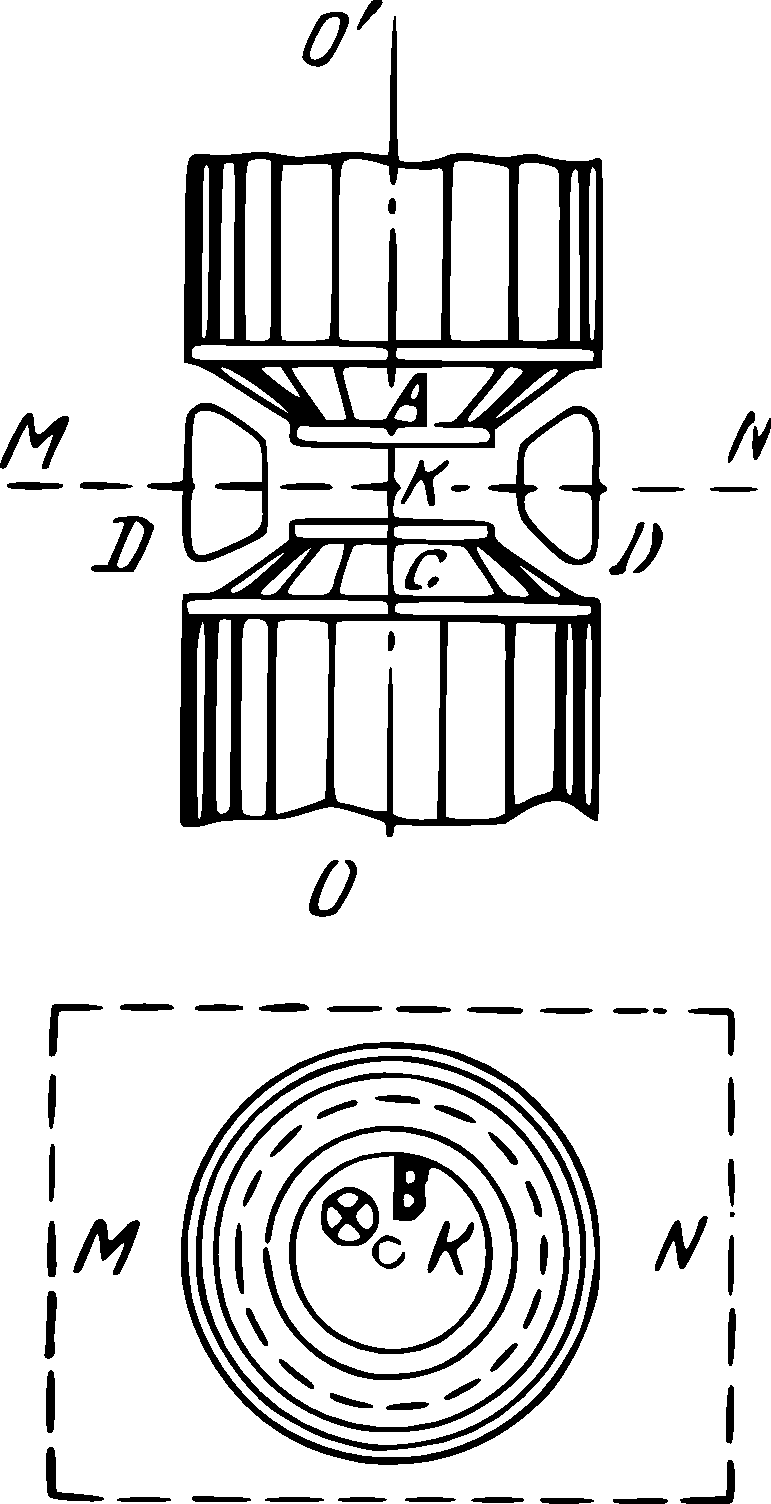
\includegraphics[width=0.8\textwidth]{figs/ch-27/fig-27-01.pdf}
\sidecaption{The working of a betatron.\zhcap{电子感应加速器的工作原理。}\label{fig-27-01}}
\end{marginfigure}

In the alternating magnetic field produced by an electromagnet with conical pole pieces $A$ and $C$ (\figr{fig-27-01}, a rotational electric field is set up in accelerating chamber $D$, having the form of a closed ring. The lines of force \ssect{15.1.6} of the rotational electric field lie in plane $MN$, which is perpendicular to the axis $OO'$ of symmetry of the pole pieces. These lines are circles with their centre at point $K$. At all points of any circle the field strength vector $\vb{E}$ has a constant numerical value and is tangent to the circle. Electrons in the accelerating chamber travel along circular paths and after repeated travel along the stable circular orbit the electron is accelerated to considerable energy.
\zhpar{在带有锥形极靴 $A$ 和 $C$ 的电磁铁所产生的交变磁场中，在呈闭合环形的加速室 $D$ 内建立了涡旋电场（见\figr{fig-27-01}）。涡旋电场的电场线（参见\ssect{15.1.6}）位于平面 $MN$ 内，该平面垂直于极靴的对称轴 $OO'$，这些电场线是以点 $K$ 为圆心的圆。在任一圆周的各点上，场强矢量 $\vb{E}$ 的数值恒定，且与该圆周相切。加速室中的电子沿圆形轨道运动，经过在稳定圆轨道上的多次运行，电子被加速到相当高的能量。}

\subsection{}\label{27.2.4} The strength $\vb{E}$ of the rotational electric field in a betatron is equal to
\zhpar{电子感应加速器中涡旋电场的场强 $\vb{E}$ 等于：}
\begin{equation*}%
E = -\frac{1}{2} r \, \dv{\expval{B}}{t} 
\end{equation*}
where $\expval{B}$ is the average value of magnetic induction at the instant of time t within the limits of the circular electron orbit of radius $r$.
\zhpar{式中 $\expval{B}$ 为时刻 $t$ 时，半径为 $r$ 的圆形电子轨道范围内磁感应强度的平均值。}

A condition for a stable orbit of the electron in the betatron is: $B = \expval{B}/2$, where $B$ is the instantaneous value of the magnetic induction on the orbit.
\zhpar{电子在电子感应加速器中稳定运行的条件是：$B = \expval{B}/2$，式中 $B$ 为轨道上磁感应强度的瞬时值。}

The orbit of an electron in the betatron is stable if:
\zhpar{电子在电子感应加速器中的轨道稳定，须满足以下两个条件：}
\begin{enumerate}[label=(\alph*)]
\item The whole orbit lies in a single plane. This condition, called \redem{axial focusing}, is achieved due to the special shape of the pole pieces of the electromagnet. This shape provides for gradual weakening of the magnetic field induction in the direction from the centre of the orbit to its periphery.
\zhpar{整个轨道位于同一平面内。这一条件称为\redem{轴向聚焦}，它是借助电磁铁特殊形状的极靴实现的。该形状使磁感应强度沿着从轨道中心指向边缘的方向逐渐减弱。}
\item Provision is made to return electrons that have accidentally left the stable orbit back to it again. This is called \redem{radial focusing} and is achieved by a space distribution of the magnetic field in which the, magnetic induction decreases more slowly from the axis to the periphery than $1/r$, where $r$ is the distance from a given point in the field to the axis of symmetry $OO'$.
\zhpar{需要采取措施，使偶然偏离稳定轨道的电子能够重新返回该轨道。这一条件称为\redem{径向聚焦}，它是借助磁场的空间分布实现的：沿从轴线到边缘的方向，磁感应强度减小得比 $1/r$ 更慢，其中 $r$ 为场中给定点到对称轴 $OO'$ 的距离。}
\end{enumerate}

\section{Displacement Current. Maxwell's Second Equation}
\label{sec-27.3}
\zhtitle{位移电流。麦克斯韦第二方程}

\subsection{}\label{27.3.1} Maxwell generalized the total current law, \ssect{26.4.2} and \ssect{26.4.4}, by assuming that a variable electric field, in the same way as an electric current, is a source of a magnetic field. The quantitative measure of the magnetic effect of a variable electric held is the displacement current.
\zhpar{麦克斯韦通过假定变化的电场与电流一样也是磁场的源，推广了全电流定律（见\ssect{26.4.2}和\ssect{26.4.4}）。变化电场磁效应的定量量度即为\redem{位移电流}。}

\subsection{}\label{27.3.2} The \redem{displacement current density} \ssect{20.2.3} is 
\zhpar{\redem{位移电流密度}（见\ssect{20.2.3}）为：}
\begin{align*}%
\vb{j}_{dis} & = \pdv{\vb{D}}{t} && \text{(in SI units),} \\
\vb{j}_{dis} & = \frac{1}{4\pi}\pdv{\vb{D}}{t}  && \text{(in Gaussian units)},
\end{align*}
The displacement current through the arbitrary surface $S$ is a physical quantity numerically equal to the flux of the displacement current density vector through this surface. Thus
\zhpar{穿过任意曲面 $S$ 的位移电流是一个物理量，其数值等于位移电流密度矢量穿过该曲面的通量。因此有：}
\begin{align*}%
{I}_{dis} & = \int_{S} \pdv{\vb{D}}{t}\,\dd \vb{S} = \pdv{\Phi_{e}}{t} && \text{(in SI units),} \\
{I}_{dis} & = \int_{S} \frac{1}{4\pi} \pdv{\vb{D}}{t}\,\dd \vb{S} = \frac{1}{4\pi} \pdv{\Phi_{e}}{t} && \text{(in Gaussian units)},
\end{align*}
where $\Phi_{e} = \int_{s} \vb{D}\, \dd \vb{S}$ is the flux of the electric displacement vector through the surface $S$ \ssect{15.3.2}.
\zhpar{式中 $\Phi_{e} = \int_{s} \vb{D}\, \dd \vb{S}$ 为穿过曲面 $S$ 的电位移矢量通量（见\ssect{15.3.2}）。}
\begin{figure}[h]%[-2cm]
\centering
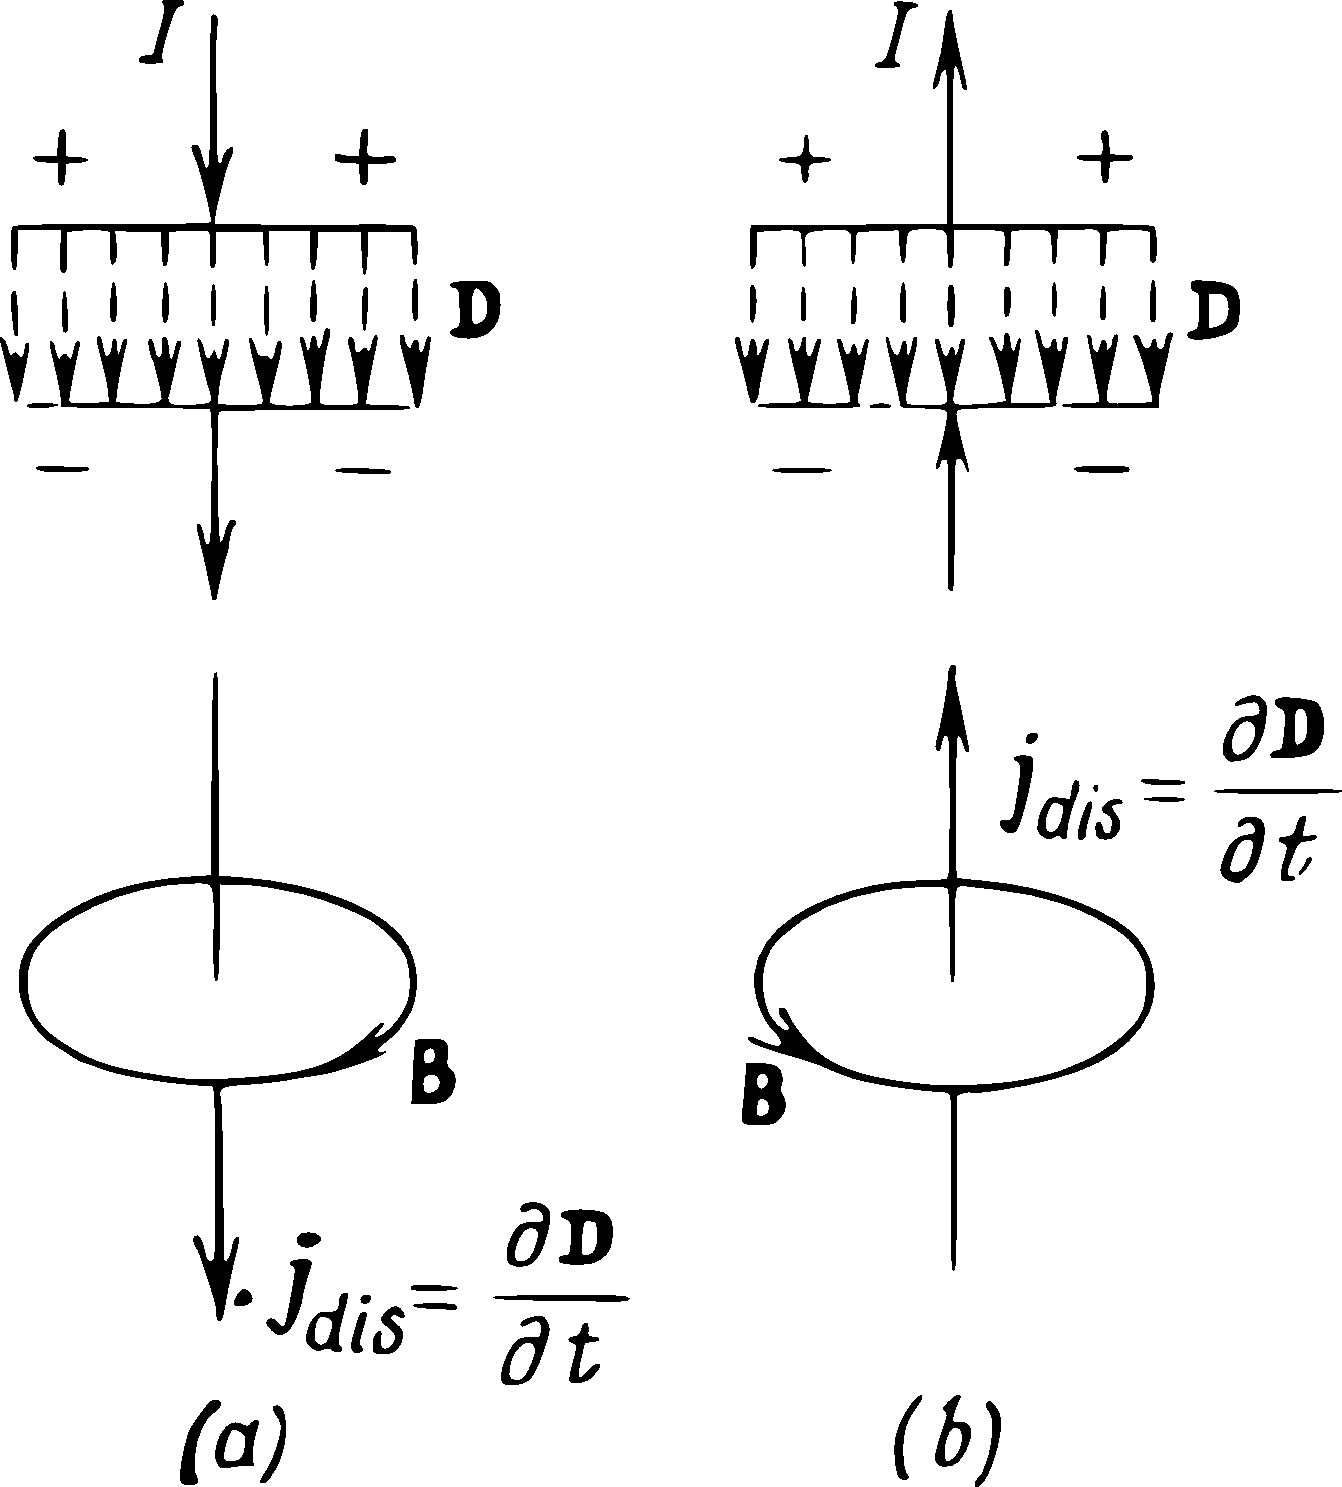
\includegraphics[width=0.7\textwidth]{figs/ch-27/fig-27-02.pdf}
\sidecaption{Understanding charging and discharging of a capacitor using the displacement current.\zhcap{利用位移电流理解电容器的充电与放电。}\label{fig-27-02}}
\end{figure}


Taking the displacement currents into account, any variable current has a closed circuit. Displacement currents ``flow'' through a part of a circuit where there is no conductor, for example, between the plates of a capacitor being charged or discharged. Shown in \figr{fig-27-02}. are the vectors j s and the lines of induction of the magnetic fields of displacement currents in charging (\figr{fig-27-02}~\drkgry{(a)}) and in discharging (\figr{fig-27-02}~\drkgry{(b)}) a capacitor. 
\zhpar{考虑位移电流之后，任何变化的电流都构成闭合回路。位移电流“流过”电路中没有导体的部分，例如正在充电或放电的电容器两极板之间。如\figr{fig-27-02}所示，给出了充电（\figr{fig-27-02}~\drkgry{(a)}）和放电（\figr{fig-27-02}~\drkgry{(b)}）电容器时矢量 j 以及位移电流磁场的磁感应线。}

\subsection{}\label{27.3.3} According to \ssect{18.3.4}, the displacement vector in any dielectric is equal to
\zhpar{根据\ssect{18.3.4}，任何电介质中的电位移矢量等于：}
\begin{align*}%
\vb{D} & = \varepsilon_{0}\vb{E} + \vb{P}_{e} && \text{(in SI units),} \\
\vb{D} & = \vb{E} + 4 \pi \vb{P}_{e}  && \text{(in cgse units)},
\end{align*}
where $\vb{P}_{e}$ is the polarization vector \ssect{18.2.3}.
\zhpar{式中 $\vb{P}_{e}$ 为极化强度矢量（见\ssect{18.2.3}）。}

The displacement current density in a dielectric is
\zhpar{电介质中的位移电流密度为：}
\begin{align*}%
\vb{j}_{dis} & = \varepsilon_{0} \pdv{\vb{E}}{t}+ \pdv{\vb{P}_{e}}{t}  && \text{(in SI units),} \\
\vb{j}_{dis} & = \frac{1}{4\pi} \pdv{\vb{E}}{t}+ \pdv{\vb{P}_{e}}{t}  && \text{(in cgse units).}
\end{align*}
In these last formulas, the first term $\varepsilon_{0} \pdv*{\vb{E}}{t}$ (or, correspondingly, $1/4\pi \, \pdv*{\vb{E}}{t}$ is called the \redem{displacement current density in vacuum},
whereas the second term $\pdv*{\vb{P}_{e}}{t} $ is called the \redem{polarization current density}. The second term is the density of the current due to the ordered motion of charges in the dielectric: either the displacement of charges in a molecule of a non-polar dielectric. \ssect{18.1.3} or the turning of the dipoles in polar dielectrics \ssect{18.1.5}. The displacement current docs not evolve Joule heal \ssect{21.2.6} in vacuum or in metals. In this it differs from conduction currents.
\zhpar{在上述最后的表达式中，第一项 $\varepsilon_{0} \pdv*{\vb{E}}{t}$（或相应的 $1/4\pi \, \pdv*{\vb{E}}{t}$）称为\redem{真空中的位移电流密度}，而第二项 $\pdv*{\vb{P}_{e}}{t}$ 称为\redem{极化电流密度}。第二项是由电介质中电荷的有序运动所引起的电流密度：它既可能是非极性电介质分子中电荷的位移（见\ssect{18.1.3}），也可能是极性电介质中偶极子的转动（见\ssect{18.1.5}）。位移电流在真空或金属中不产生焦耳热（见\ssect{21.2.6}）。在这一点上，它与传导电流不同。}

\subsection{}\label{27.3.4} Maxwell added the displacement current to the right- hand side of the. total current law in the form given in \ssect{26.4.4}, writing this law in the form
\zhpar{麦克斯韦将位移电流加到全电流定律的右端（其形式与\ssect{26.4.4}中所给出的一致），并将该定律写为：}
\begin{align*}%
\oint_{L} \vb{H} \, \dd \vb{l} & = I_{mac} + I_{dis}  && \text{(in SI units),} \\
\oint_{L} \vb{H} \, \dd \vb{l} & = \frac{4 \pi}{c}(I_{mac} + I_{dis}) && \text{(in Gaussian units).}
\end{align*}
This equation is called \redem{Maxwell's second equation in integral form}. It shows that the circulation of the magnetic field strength vector along an arbitrary closed circuit, or loop, L is equal to the algebraic sum of the macro-currents and the displacement current through a surface bounded by this loop.
\zhpar{该方程称为\redem{麦克斯韦第二方程的积分形式}。它表明：磁场强度矢量沿任一闭合回路 $L$ 的环流，等于以该回路为边界的曲面所穿过的宏观电流与位移电流的代数和。}

\subsection{}\label{27.3.5} Making use of the Stokes theorem from vector analysis
\zhpar{利用矢量分析中的斯托克斯定理：}
\begin{equation*}%
\oint_{L} \vb{H} \, \dd \vb{l}  = \oint_{S} \curl \vb{H} \, \dd \vb{S}
\end{equation*}
where $\dd \vb{S} = \vu{N} \dd S$, and $\vu{n}$ is a unit vector of the normal to the element $\dd S$ of surface, and of the expression for the total current
\zhpar{式中 $\dd \vb{S} = \vu{N} \dd S$，$\vu{n}$ 为面元 $\dd S$ 的法线单位矢量，并利用全电流的表达式：}
\begin{equation*}%
I = I_{mac} + I_{dis} = \int_{S} (\vb{j} + \vb{j}_{dis}) \, \dd \vb{S}
\end{equation*}
\zhpar{麦克斯韦第二方程的微分形式可写为：}
Maxwell's second equation can be written in differential form: \begin{align*}%
\curl \vb{H} & = \vb{j} + \pdv{\vb{D}}{t} && \text{(in SI units),} \\
\oint_{L} \vb{H} \, \dd \vb{l} & = \frac{4 \pi}{c}(I_{mac} + I_{dis}) && \text{(in Gaussian units).}
\end{align*}
In these equations, $\curl \vb{H}$ has the same meaning as $\curl \vb{E}$ in \ssect{27.2.2}.
\zhpar{在这些方程中，$\curl \vb{H}$ 的含义与\ssect{27.2.2}中 $\curl \vb{E}$ 的含义相同。}

\subsection{}\label{27.3.6} In the absence of conduction currents $(\vb{j} = 0)$, Maxwell's first and second equations are of symmetrical form except for sign in their right-hand sides:
\zhpar{在没有传导电流（$\vb{j} = 0$）的情况下，麦克斯韦第一方程与第二方程的形式除右端符号外是对称的：}
\begin{align*}%
\curl \vb{E} & = \pdv{\vb{B}}{t}, \, \curl \vb{H} = \pdv{\vb{D}}{t} && \text{(in SI units),} \\
\curl \vb{E} & = -\frac{1}{c} \pdv{\vb{B}}{t}, \, \curl \vb{H} = \frac{1}{c}  \pdv{\vb{D}}{t} && \text{(in Gaussian units).}
\end{align*}
Comparing Maxwell's equations\sidenote{The numeration of Maxwell's equations is a conditional one and is frequently the opposite of that accepted in this handbook.}, we reach the following conclusions:
\zhpar{比较麦克斯韦方程组，可以得出以下结论：}
\zhpar{注：麦克斯韦方程的编号是约定的，常与本手册所采用的编号相反。}
\begin{enumerate}[label=(\alph*)]
\item Electric and magnetic fields are interrelated: a change of an electric field with time sets up a magnetic field\sidenote{The magnetic field is always a rotational one \ssect{23.5.3}.}. In its turn, a variable magnetic field is the source of a rotational electric field.
\zhpar{电场与磁场相互联系：电场随时间的变化激发磁场。反过来，变化的磁场是涡旋电场的源。}
\zhpar{注：磁场总是涡旋场（参见\ssect{23.5.3}）。}
\item The different signs at the right-hand sides of Maxwell's equations comply with the law of conservation of energy and with the Lenz law \ssect{25.1.4}. If the signs of $\pdv*{\vb{B}}{t}$ and $\pdv*{\vb{D}}{t}$ were the same, an infinitesimal increase in one of the fields would lead to an increase without limit of both fields, whereas an infinitesimal decrease in one of the fields would lead to the disappearance of both fields. The above-mentioned difference in the signs of the right-hand (a) sides of Maxwell's equations is a necessary condition for the existence of a stable electromagnetic field.
\zhpar{麦克斯韦方程右端符号的上述差异符合能量守恒定律，也符合楞次定律（见\ssect{25.1.4}）。若 $\pdv*{\vb{B}}{t}$ 与 $\pdv*{\vb{D}}{t}$ 的符号相同，则场的任一无穷小增加都将导致两者无限增大，而场的任一无穷小减小都将导致两者同时消失。因此，麦克斯韦方程右端符号的差异是电磁场稳定存在的必要条件。}
\end{enumerate}

\begin{marginfigure}[-4cm]
\centering
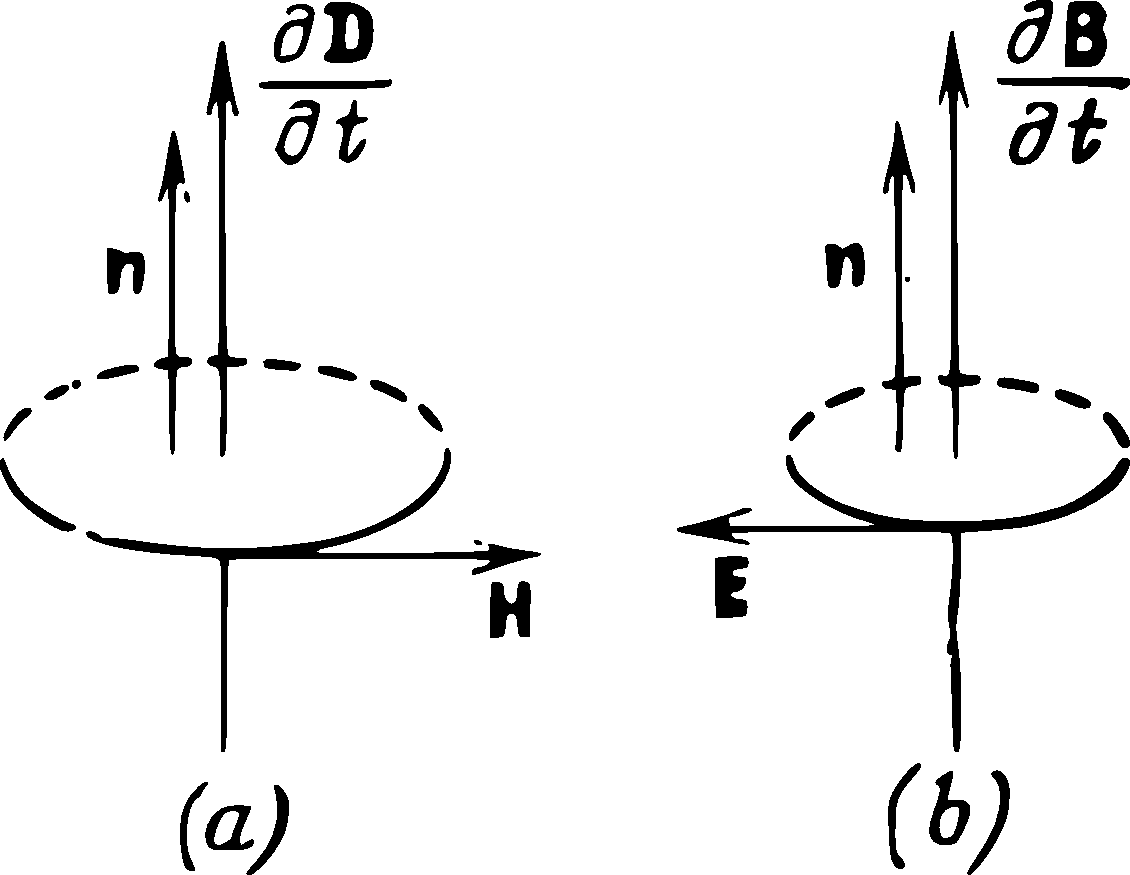
\includegraphics[width=0.8\textwidth]{figs/ch-27/fig-27-03.pdf}
\sidecaption{Relationship between quantities in Maxwell's equations.\zhcap{麦克斯韦方程中各量之间的关系。}\label{fig-27-03}}
\end{marginfigure}

The different signs in the right-hand sides of Maxwell's equations correspond to the fact that the directions of $\pdv*{\vb{D}}{t}$ and $\vb{H}$ form a ``right-hand screw'' system (\figr{fig-27-03}~\drkgry{(a)}), whereas the directions of $\pdv*{\vb{B}}{t}$ and $\vb{E}$ form a ``left-hand screw'' system (\figr{fig-27-03}~\drkgry{(b)}).
\zhpar{麦克斯韦方程右端符号的不同，对应于以下事实：$\pdv*{\vb{D}}{t}$ 与 $\vb{H}$ 的方向构成“右手螺旋”系统（见\figr{fig-27-03}~\drkgry{(a)}），而 $\pdv*{\vb{B}}{t}$ 与 $\vb{E}$ 的方向构成“左手螺旋”系统（见\figr{fig-27-03}~\drkgry{(b)}）。}


\section[Complete Set of Maxwell's Equations]{Complete Set of Maxwell's Equations for an Electromagnetic Field}
\label{sec-27.4}
\zhtitle{电磁场的完整麦克斯韦方程组}


\subsection{}\label{27.4.1} A complete set of Maxwell's equations for an electromagnetic field includes, in addition to the equations dealt with in sections \ssect{27.2.1}, \ssect{27.2.2}, \ssect{27.3.4} and \ssect{27.3.5}, the Ostro-gradsky-Gauss theorem for an electric field \ssect{18.3.3}:
\zhpar{电磁场的完整麦克斯韦方程组除包括\ssect{27.2.1}、\ssect{27.2.2}、\ssect{27.3.4}和\ssect{27.3.5}中讨论的方程外，还包括电场的奥斯特罗格拉茨基-高斯定理（见\ssect{18.3.3}）：}
\begin{equation*}%
\oint_{S } \vb{D} \dd \vb{S}  = 4 \pi q_{\textrm{free}} \quad \text{in cgse units}
\end{equation*}
and the same theorem for a magnetic field \ssect{23.5.6}:
\zhpar{以及磁场的同一定理（见\ssect{23.5.6}）：}
\begin{equation*}%
\oint_{S } \vb{B} \dd \vb{S}  = 0 \quad \text{in cgse units}
\end{equation*}
Maxwell proposed that the theorem for the flux of an electric field displacement vector is valid, not only for a steady-state electrostatic field, but for a variable electric field as well. 
\zhpar{麦克斯韦提出，电位移矢量通量的定理不仅对稳恒静电场成立，对变化的电场同样成立。}

\subsection{}\label{27.4.2} Making use of the Gauss theorem from vector analysis:
\zhpar{利用矢量分析中的高斯定理（即散度定理）：}
\begin{equation*}%
\oint_{S} \vb{A} \dd \vb{S}  = \int_{V} \div \vb{A} \, \dd V, 
\end{equation*}
and introducing the volume density $\rho$ of free charges: $\rho = \dd q_{\textrm{free}}/\dd V$ (where $\dd V$ is an element of volume), it is possible to obtain \redem{Maxwell's third equation in differential form}:
\zhpar{引入自由电荷的体密度 $\rho$：$\rho = \dd q_{\textrm{free}}/\dd V$（其中 $\dd V$ 为体积元），由此可得到\redem{麦克斯韦第三方程的微分形式}：}
\begin{align*}%
\div \vb{D} & = \rho && \text{(in SI units),} \\
\div \vb{D} & = 4 \pi \rho && \text{(in Gaussian units),}
\end{align*}
In these equations, $\div \vb{A}$ (where $\vb{A}$ is an arbitrary vector) is determined in Cartesian coordinates as follows:
\zhpar{在这些方程中，$\div \vb{A}$（其中 $\vb{A}$ 为任意矢量）在笛卡儿直角坐标系中按如下方式确定：}
\begin{equation*}%
\div \vb{A}= \pdv{A_{x}}{x} + \pdv{A_{y}}{y}  + \pdv{A_{z}}{z}, 
\end{equation*}
where $\vb{A} = A_{x} \vu{i}+ A_{y} \vu{j} + A_{z} \vu{k}$ and $\vu{i}$, $\vu{j}$, and $\vu{k}$ are unit vectors along the coordinate axes.
\zhpar{式中 $\vb{A} = A_{x} \vu{i}+ A_{y} \vu{j} + A_{z} \vu{k}$，$\vu{i}$、$\vu{j}$ 和 $\vu{k}$ 为沿坐标轴方向的单位矢量。}

\subsection{}\label{27.4.3} The \redem{complete set of Maxwell's equations} includes four equations:
\zhpar{\redem{完整的麦克斯韦方程组}包括四个方程：}
\begin{align*}%
\curl \vb{E} & = - \pdv{\vb{B}}{t},\,\, &\div \vb{D} & = \rho, && \text{(in SI units),} \\
\curl \vb{H} & = \vb{j} + \pdv{\vb{D}}{t},\,\, &\div \vb{B} & = 0, && \text{(in SI units),} \\
\curl \vb{E} & = - \frac{1}{c} \pdv{\vb{B}}{t},\,\, &\div \vb{D} &= 4 \pi \rho, && \text{(in Gaussian units),} \\
\curl \vb{H} & = \frac{4\pi}{c}\vb{j} + \frac{1}{c}\pdv{\vb{D}}{t},\,\, &\div \vb{B} &= 0,  && \text{(in Gaussian units).}
\end{align*}

\subsection{}\label{27.4.4} The system of Maxwell's equations is supplemented by equations that specify the electric and magnetic properties of the medium. For macro-currents in an isotropic medium, which comply with Ohm's law \ssect{20.3.4}, these equations are of the form
\zhpar{麦克斯韦方程组还需补充描述介质电学和磁学性质的方程。对于遵从欧姆定律（见\ssect{20.3.4}）的各向同性介质中的宏观电流，这些方程的形式为：}
\begin{align*}%
\vb{D} & = \varepsilon_{0}\varepsilon_{r} \vb{E}, \,\, \vb{B} = \mu_{0}\mu_{r} \vb{H} \,\, \vb{j}_{mac} = \varkappa \vb{E} && \text{(in SI units),} \\
\vb{D} & = \varepsilon_{r} \vb{E}, \,\, \vb{B} = \mu_{r} \vb{H} \,\, \vb{j}_{mac} = \varkappa \vb{E} && \text{(in Gaussian units).}
\end{align*}
Here $\varepsilon_{0}$ and $\mu_{0}$ are the electric constant \ssect{14.2.7} and the magnetic constant \ssect{23.2.2} in SI units, $\varepsilon_{r}$ and $\mu_{r}$ are the relative dielectric constant and relative magnetic permeability, and x is the electrical conductivity.
\zhpar{式中，$\varepsilon_{0}$ 和 $\mu_{0}$ 分别为SI单位制中的电常量（见\ssect{14.2.7}）与磁常量（见\ssect{23.2.2}），$\varepsilon_{r}$ 和 $\mu_{r}$ 分别为相对介电常量与相对磁导率，$\varkappa$ 为电导率。}

To solve a system of Maxwell's equations, it is also necessary to specify the boundary conditions for the vectors characterizing the electromagnetic field. Thus
\zhpar{为求解麦克斯韦方程组，还需给出表征电磁场的矢量的边界条件。具体而言：}
\begin{align*}%
D_{n_{1}} - D_{n_{2}}& = \sigma,\,\, & E_{t_{1}} & = E_{t_{2}}, \\ &  \text{(in SI units),} \\
B_{n_{1}} & = B_{n_{2}},\,\, & H_{t_{1}}-H_{t_{2}} & =  j_{sur}, \\ & \text{(in SI units),} \\
D_{n_{1}} - D_{n_{2}} & = 4\pi\sigma,\,\, & E_{t_{1}} & = E_{t_{2}}, \\ & \text{(in Gaussian units),} \\
B_{n_{1}} & = B_{n_{2}},\,\, & H_{t_{1}}-H_{t_{2}} & =  \frac{4\pi}{c}j_{sur}, \\ &  \text{(in Gaussian units).}
\end{align*}
where $\sigma$ is the surface density of free charges, $\vu{n}$ is a unit vector of the normal to the interface (boundary) between media and extends from medium $\mathcal{2}$ to medium $\mathcal{1}$, $\vu{t}$ is a unit vector of the tangent to the interface, and $j_{sur}$ is the projection of the density vector of surface conduction currents on the direction $[\vu{t}\,\vu{n}]$. For given boundary and initial conditions, i.e. known values of vectors $\vb{E}$ and $\vb{H}$ at the initial instant of time $(t=0)$ the system of Maxwell's equations has a unique solution.
\zhpar{式中 $\sigma$ 为自由电荷的面密度，$\vu{n}$ 为介质分界面（边界）法线方向的单位矢量，其方向由介质 $\mathcal{2}$ 指向介质 $\mathcal{1}$；$\vu{t}$ 为分界面切线方向的单位矢量；$j_{sur}$ 为面传导电流密度矢量在方向 $[\vu{t}\,\vu{n}]$ 上的投影。在给定边界条件和初始条件，即已知初始时刻 $(t=0)$ 矢量 $\vb{E}$ 和 $\vb{H}$ 的值时，麦克斯韦方程组有唯一解。}

\subsection{}\label{27.4.5} Maxwell's equations are invariant with respect to the Lorentz transformations \ssect{5.3.2}.
\zhpar{麦克斯韦方程组在洛伦兹变换下是不变的（见\ssect{5.3.2}）。}

In the special theory of relativity \ssect{5.1.1} it is shown that a common electromagnetic field can be different in different inertial frames of reference \ssect{2.1.2}. In particular, one of the fields, either electric or magnetic, may be absent in one of the coordinate systems and be present in the other. The following formulas are used for the Lorentz transformations of the projections on the coordinate axes of the vectors $\vb{E}$, $\vb{H}$, $\vb{D}$ and $\vb{B}$ of the electric and magnetic fields, in going over from fixed inertial frame of reference $K$ to frame $K'$ which travels with respect to frame $K$ at the constant velocity $V$ in a straight line along the $OX$ axis:
\zhpar{狭义相对论（见\ssect{5.1.1}）指出，同一电磁场在不同的惯性参考系（见\ssect{2.1.2}）中可以不同。特别地，电场和磁场中的一种可能在某一坐标系中不存在，而在另一坐标系中存在。在由固定惯性参考系 $K$ 过渡到相对于 $K$ 沿 $OX$ 轴以恒定速度 $V$ 做直线运动的参考系 $K'$ 时，电场与磁场矢量 $\vb{E}$、$\vb{H}$、$\vb{D}$ 和 $\vb{B}$ 在坐标轴上投影的洛伦兹变换公式如下：}
\begin{align*}%
E_{x}& = E_{x}',\,\, & E_{y} & = \gamma(E_{y}'+ VB_{z}'), & E_{z} & = \gamma(E_{z}'- VB_{y}'), && \text{(in SI units),} \\
H_{x}& = H_{x}',\,\, & H_{y} & = \gamma(H_{y}' - VD_{z}'), & H_{z} & = \gamma(H_{z}'+ VD_{y}'), && \text{(in SI units),} \\
D_{x}& = D_{x}',\,\, & D_{y} & = \gamma \left(D_{y}' + \frac{\beta}{c}H_{z}' \right), & D_{z} & = \gamma \left(D_{z}' + \frac{\beta}{c}H_{y}' \right), && \text{(in Gaussian units),} \\
B_{x}& = B_{x}',\,\, & B_{y} & = \gamma \left(B_{y}' - \frac{\beta}{c}E_{z}' \right), & B_{z} & = \gamma \left(B_{z}' + \frac{\beta}{c}E_{y}' \right), && \text{(in Gaussian units),} \\
E_{x}& = E_{x}',\,\, & E_{y} & = \gamma \left(E_{y}' + \beta \, H_{z}' \right), & E_{z} & = \gamma \left(E_{z}' + \beta \, H_{y}' \right), && \text{(in Gaussian units),} \\
H_{x}& = H_{x}',\,\, & H_{y} & = \gamma \left(H_{y}' - \beta \, E_{z}' \right), & H_{z} & = \gamma \left(H_{z}' + \beta \, E_{y}' \right), && \text{(in Gaussian units).}
\end{align*}
Where $\beta = V/c$ and $\gamma = 1/\sqrt{1 - V^{2}/c^{2}}$.
\zhpar{其中 $\beta = V/c$，$\gamma = 1/\sqrt{1 - V^{2}/c^{2}}$。}

\subsection{}\label{27.4.6} The classical Lorentz theory of the electron is a further development of Maxwell's theory of the electromagnetic field.
\zhpar{经典洛伦兹电子论是麦克斯韦电磁场理论的进一步发展。}

The Lorentz theory is based on a definite model that implies certain conceptions of the structure of matter. It is assumed that atoms consist of negatively and positively charged particles, and that the great variety of electrical and magnetic phenomena can be explained by a definite spatial arrangement, motion and interaction of charges and micro-currents. At each point in space certain electric and magnetic micro-fields exist with the strengths $\vb{e}$ and $\vb{h}$. These fields result from the combined action of all the charges and micro-currents. The micro-fields comply with a system of equations similar to Maxwell's equations \ssect{27.4.3}. Maxwell's equations for macroscopic fields E and B \ssect{27.1.3} can be obtained by averaging the equations of the electron theory \ssect{27.1.4}, and they are found to be the averaged microfields e and h. Thus
\zhpar{洛伦兹理论基于一定的模型，该模型包含关于物质结构的某些设想。假定原子由带负电和带正电的粒子组成，各种各样的电现象和磁现象可以由电荷与微电流的确定的空间分布、运动及相互作用来解释。空间中各点存在具有场强 $\vb{e}$ 和 $\vb{h}$ 的微观电场与微观磁场，这些微观场是所有电荷与微电流共同作用的结果。微观场遵从与麦克斯韦方程组（见\ssect{27.4.3}）相似的一组方程。对电子理论的方程取平均（见\ssect{27.1.4}），即可得到宏观场 E 和 B 所满足的麦克斯韦方程（见\ssect{27.1.3}），且宏观场 E 和 B 恰好就是对微观场 $\vb{e}$ 和 $\vb{h}$ 取平均的结果。于是有：}
\begin{equation*}%
\vb{E} = \expval{\vb{e}},\,\, \vb{B} = \mu_{0}\expval{\vb{h}} \quad \text{(in SI units).}
\end{equation*}
Vectors $\vb{D}$ and $\vb{H}$ are found to be related to $\expval{\vb{e}}$ and $\expval{\vb{h}}$ by the polarization vector $\vb{P}_{e}$ \ssect{18.2.3} and the magnetization vector $\vb{M}$ \ssect{26.3.1} as indicated in \ssect{18.3.4} and \ssect{26.4.4}. Thus
\zhpar{如\ssect{18.3.4}和\ssect{26.4.4}中所示，矢量 $\vb{D}$ 和 $\vb{H}$ 分别通过极化强度矢量 $\vb{P}_{e}$（见\ssect{18.2.3}）和磁化强度矢量 $\vb{M}$（见\ssect{26.3.1}）与平均微观场 $\expval{\vb{e}}$ 和 $\expval{\vb{h}}$ 相联系。于是有：}
\begin{align*}%
\vb{D} & = \varepsilon_{0} \vb{E}, + \vb{P}_{e},\,\, & \vb{H} & =\frac{\vb{B}}{\mu_{0}} - \vb{M}, && \text{(in SI units),} \\
\vb{D} & =  \vb{E}, + 4 \pi \vb{P}_{e},\,\, & \vb{H} & =\vb{B} - 4 \pi \vb{M}, && \text{(in Gaussian units).}
\end{align*}



